\section{Unit tests}

We have utilized the unittest package for Python to ensure good quality in our backend. By creating a comprehensive suite of unit tests, we are able to systematically test individual units of code in isolation, ensuring that each function and method works as expected. 

To ensure that our unit tests cover as much of the codebase as possible, we have also utilized the coverage package for Python. This package allows us to measure how much our unit tests exercise the codebase. By analyzing the results of code coverage reports, we can identify areas of the codebase that are not being tested and prioritize efforts to improve test coverage.

On the frontend side, we utilized the Jest testing framework as our unit test package for TypeScript. Jest is a popular testing framework used for testing Vue applications and is highly regarded for its ease of use and powerful features. Since Jest already includes coverage we didn't need another framework in the frontend.

Overall we achieved $\geq 90 \%$ code coverage on both front and backend as documented in the following pictures. 

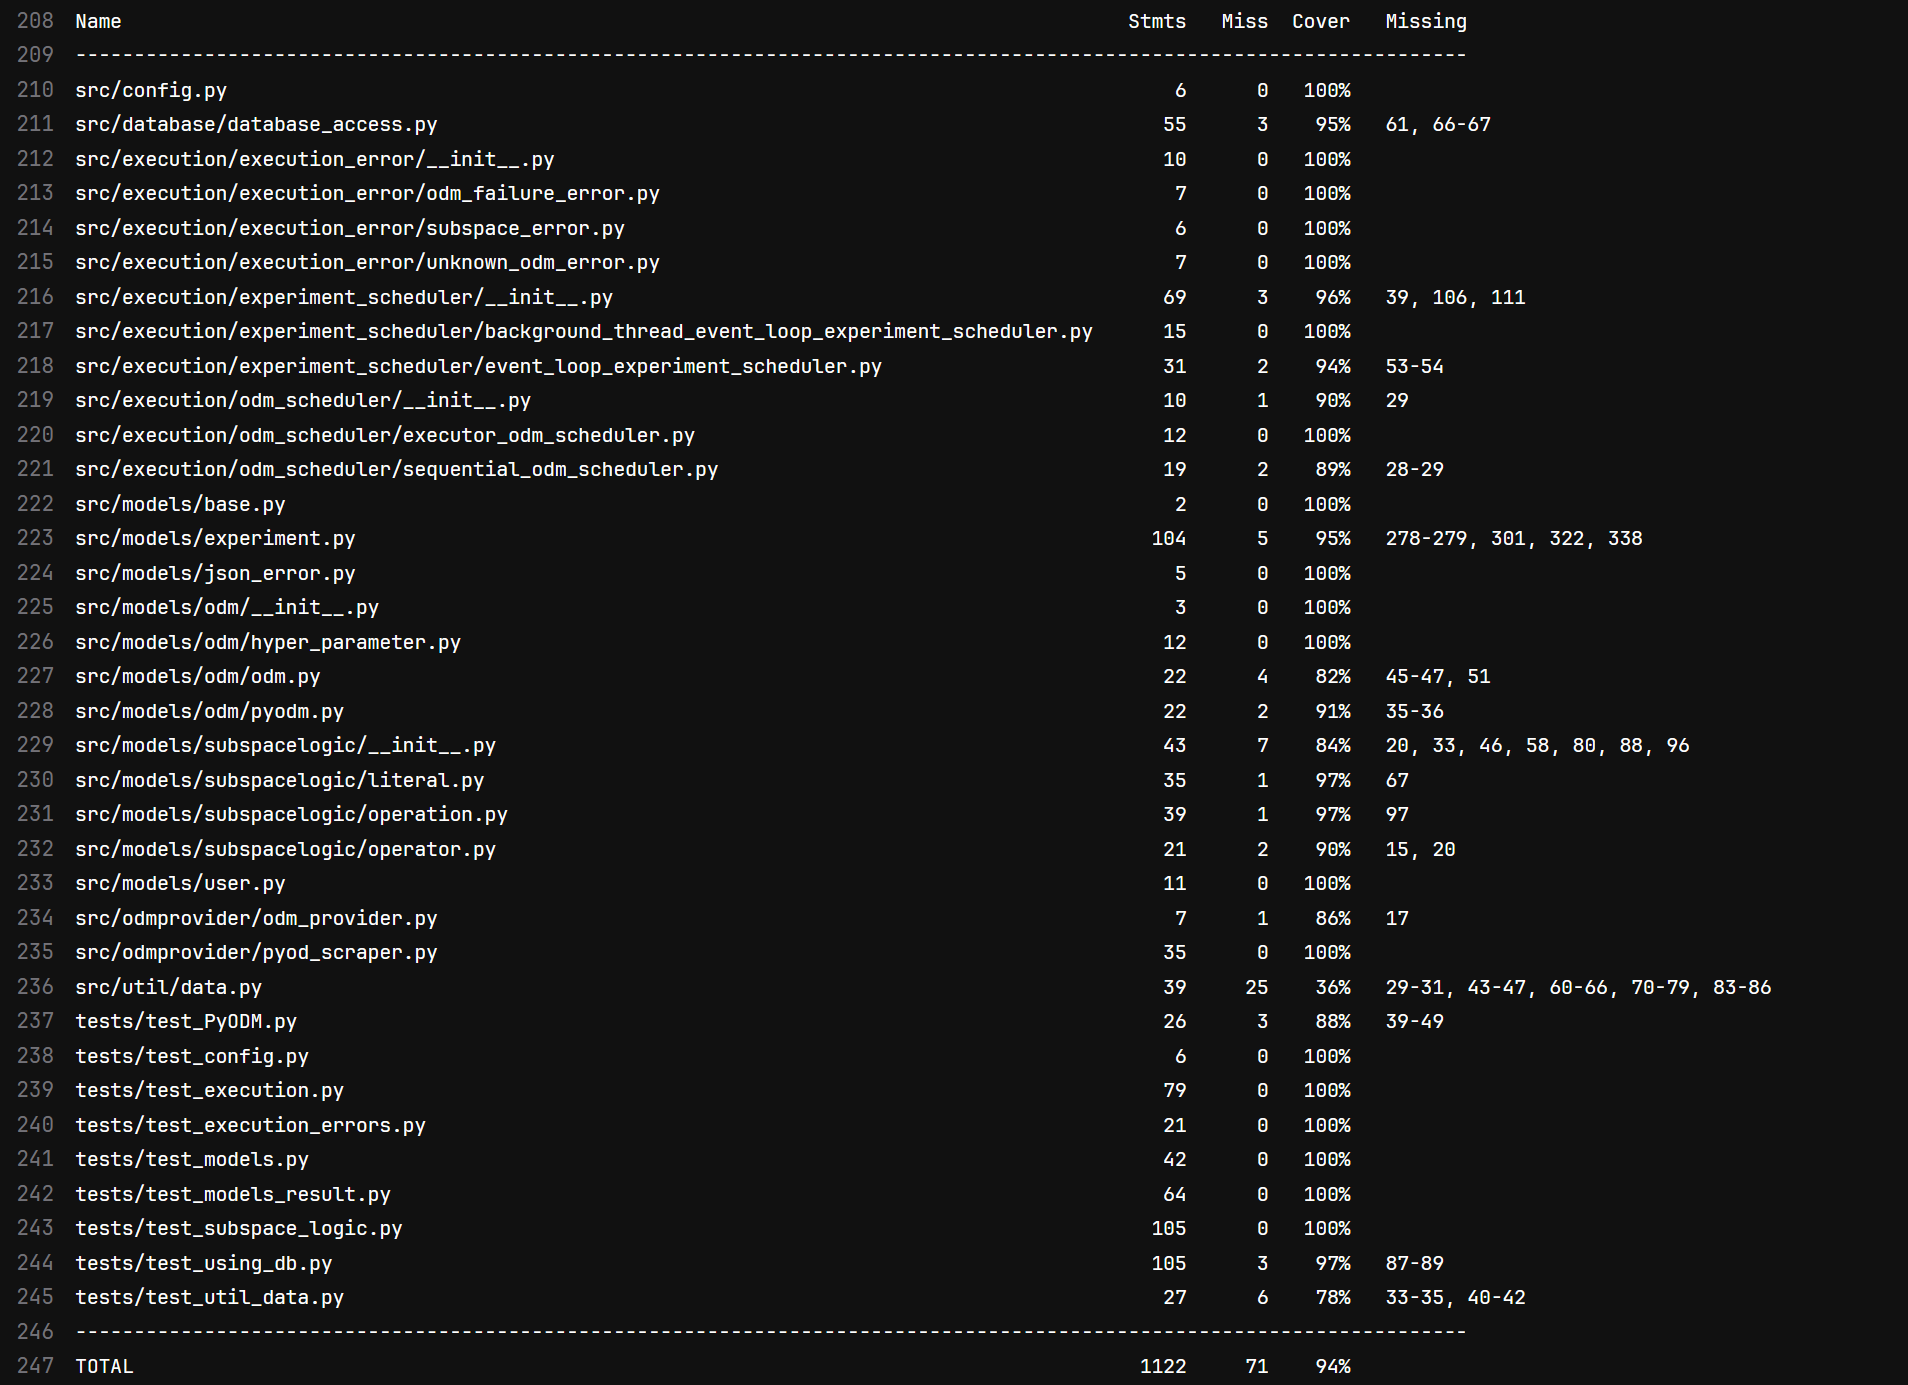
\includegraphics[width=1\textwidth]{images/backend.png}
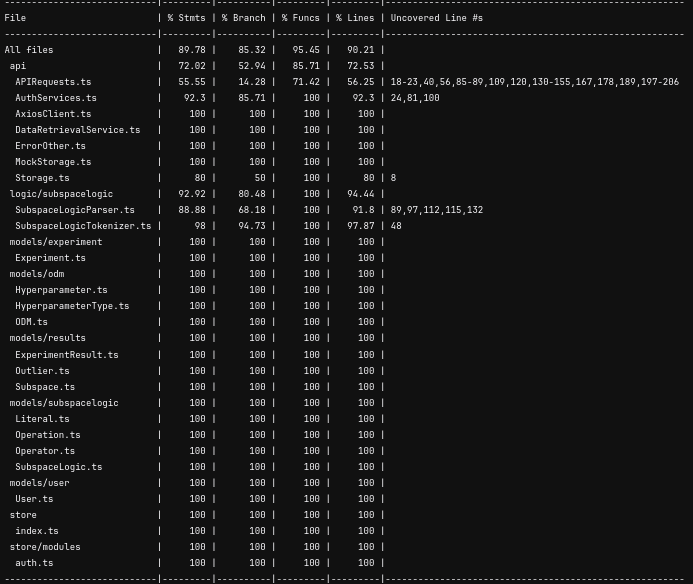
\includegraphics[width=1\textwidth]{images/frontend.png}
